% Document template based on LNCS, adapted by Matt Welsh <mdw@cs.berkeley.edu> and Mark Hempstead<mhempstead@coe.drexel.edu>

% This version is adapted to use PDFTEX to render to PDF directly. 
% If you want to use dvi, you need to change any figures to use '.eps'
% rather than '.pdf', and probably get rid of the hyperref package.

\documentclass{article}
\usepackage{program}
\usepackage{acm-style10} % ACM proceedings formatting
\usepackage{times}       % Use Adobe Times font set
\usepackage{epsfig,twocolumn}
\usepackage{url}
\usepackage[english]{babel} % mdw: Required to get good hyphenation on RH6.0
                            % (fixed in RH6.1)
\usepackage{graphicx} 
\usepackage{color}

% DO NOT EDIT THE BELOW BLOCK OF CODE
\def\dsp{\def\baselinestretch{1.10}}
\dsp
\newcommand{\XXXnote}[1]{{\bf\color{red} XXX: #1}}
\setlength{\textheight}{9.25in}
\setlength{\columnsep}{0.33in}
\setlength{\textwidth}{7.4in}
\setlength{\footskip}{0.0in}
\setlength{\topmargin}{-0.25in}
\setlength{\headheight}{0.0in}
\setlength{\headsep}{0.0in}
\setlength{\oddsidemargin}{-.45in}
\setlength{\parindent}{1pc}
\pagestyle{empty}
\begin{document}
\date{}

%%%%%%%%%%%% THIS IS WHERE WE PUT IN THE TITLE AND AUTHORS %%%%%%%%%%%%

% Title here
\title{\ttlfnt EE 194 Project Paper}

% Author names, affiliations, and e-mail below
\author{{\aufnt   Xu Liu } \\ 
{\affaddr Tufts University} \\ 
{\affaddr     xu.liu@tufts.edu }}

\maketitle
%\copyrightspace
\thispagestyle{empty}

%%%%%%%%%%%%%  ABSTRACT GOES HERE %%%%%%%%%%%%%%

\subsection*{Abstract}
\begin{small}
Our final project is comparing performances of CPU and GPU by implementing
several sorting algorithms respectively on GPU in sequential way and on GPU
in parallel way.
\end{small}

%%%%%%%%%%%%%  BODY OF PAPER GOES HERE %%%%%%%%%%%%%%

% Generally you will want to break the paper into separate sections
% and use \input{...} to include them, like so:
%\input{intro.tex} 
%\input{motivation.tex}
%\input{design.tex}
%\input{implementation.tex}
%\input{evaluation.tex}
%\input{conclusion.tex}
\section*{}

\section{Introduction}

 Since we have hit the power wall and memory wall on the road of improving computers' performance by continually increasing the frequency of
 processor, we are exploring other ways to keep the performance of computer growing while keep the CPU cool. These ways include making more CPU on single chip, exploiting GPU or AISC's, dynamically adjusting voltage and frequency and so on.\\
GPU probably will be very helpful for improving integrated performance of the whole computer system. Therefore people usually care about
how GPU benefits the overall performance and what kind of programming model helps.
 

\section{Project Description}
This project is comparing absolute performances of CPU and GPU on sorting algorithms.
\begin{itemize}

\item \textbf{Platform} Our programs are developed on the computer in lab 120, which has CPU: intel Core i5 at 3.3 GHz, GPU: Nvidia k620 at 1.124Gh with 2 G  GPU memory.

\item \textbf{Algorithms} We implemented five sequential sorting algorithms : shell, merge, quick, insertion and radix sorting; we also implemented three parallel algorithms: merge, even odd and bitonic sorting. In addition we call parallel radix sorting directly from Nvidia library--thrust as a reference.
\item \textbf{Tools}  We use \textit{ nvcc} compile our programs. We use program \textit{time} to measure the consuming time. It will report the total time consuming, time consumed by system and the time consumed by our application. We use another tool \textit{Nvidia Visual Profiler} to profile our program and get details about
each module.
\end{itemize} 

 



\section{Experimental Methodology}

 \begin{enumerate}
	\item We implement all five sequential sorting algorithms to provide a reference for later comparisons.
	\item We write simple cuda program to test the platform and system and obtain detailed system information.
	\item We develop the three parallel algorithms one each step.
	\item We write scripts to measure time consuming of each algorithms on different data set.
	\item We plot chart on the test results while comparing the test results.
	\item We profile each parallel algorithms to analyze the reason why some are faster than the others.
 \end{enumerate}
 



\section{Results and Analysis}
\label{sec:results}  %labels are useful if you want to be able to refer to sections in other places in the text.

 
\begin{figure}[t]
\begin{center}
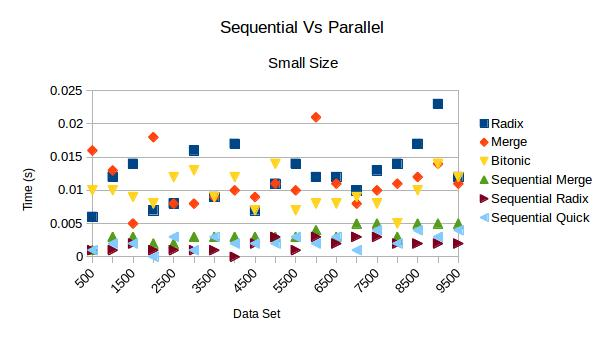
\includegraphics[width=0.8\hsize]{./figures/sVp_s.jpg}
\end{center}
\caption{{\small {\bf Comparison between sequential and parallel sorting on small size data set.} }}
\label{fig-knearest-perf}
\end{figure}
 
Figure 1 shows, for small size data set (less than 10000 elements), there is no obvious trend and also no big difference between different sorting algorithms.\\
\begin{figure}[t]
\begin{center}
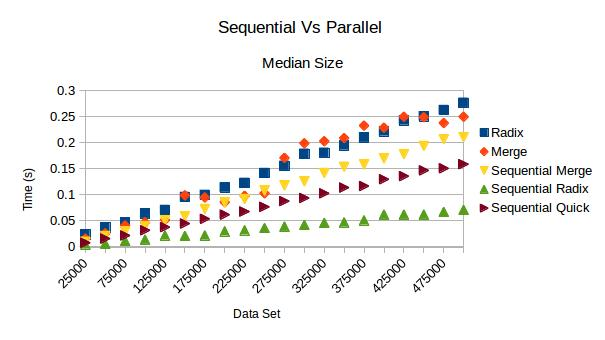
\includegraphics[width=0.8\hsize]{./figures/sVp_m.jpg}
\end{center}
\caption{{\small {\bf Comparison between sequential and parallel sorting on median size data set.} {\em This figure shows, for median size data set (between tens of thousands and million),  sequential outperforms parallel.}}}
\label{fig-knearest-perf}
\end{figure}For median and large size data set, sequential sorting outperforms parallel sorting as shown in Figure 2 and 3. This result was not expected by us.
\section*{}
Figure 4 is the summary of our comparison results.
This is the first time we program on GPU and also first time use cuda.  We think the reason why the sequential sorting are so fast is that CPU has been optimized well enough by pipeline, branch prediction, cache policy and so on. Well why the parallel sorting are slow? We continue to profile all the parallel to see details.
\begin{figure}[t]
\begin{center}
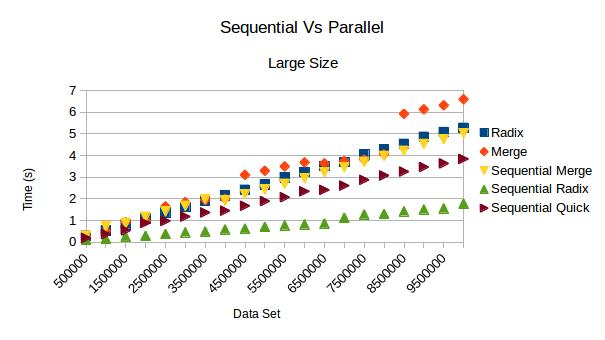
\includegraphics[width=0.8\hsize]{./figures/sVp_l.jpg}
\end{center}
\caption{{\small {\bf Comparison between sequential and parallel sorting on large size data set.} {\em This figure shows, for large size data set (between millions and tens of millions),  sequential outperforms parallel.}}}
\label{fig-knearest-perf}
\end{figure}
\section*{}
Figure 5 is the profiling for parallel radix.
Parallel radix sort comes from Nvidia thrust library, therefore we are not very familiar with its structure. The profiling shows that it is
very compact and exploit the shared memory well. However it still can not outperform sequential radix sort.
\section*{}
Radix is kind of data independent, we can keep multiple threads on data set.
It only visit memory one or two times for each element.
Actually it possesses a programming model which  fit in GPU very well except it may need dynamically allocate memory.
data independent. We probably can improve it .
\begin{figure}[t]
\begin{center}
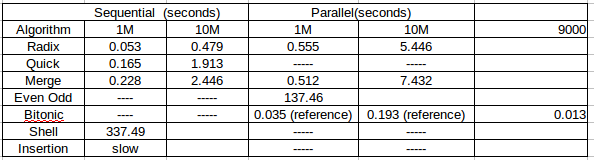
\includegraphics[width=0.8\hsize]{./figures/summary.png}
\end{center}
\caption{{\small {\bf Summary for comparison between sequential algorithms and parallels.}  }}
\label{fig-knearest-perf}
\end{figure}

\section*{}

Figure 6 tells us that the last few rounds of parallel merge sort only use few threads and therefore consume most of the time. We think the 
reason it is slow is that this strategy cannot exploit multiple threads well enough.\\
\begin{figure}[t]
\begin{center}
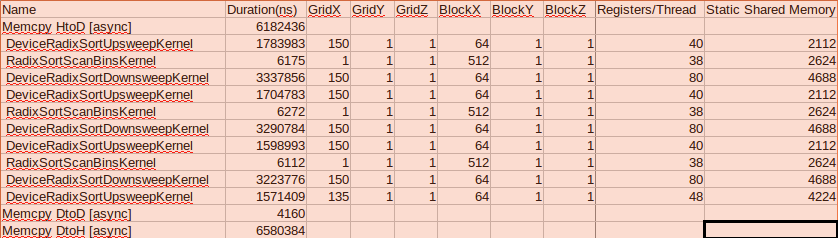
\includegraphics[width=0.8\hsize]{./figures/radix.png}
\end{center}
\caption{{\small {\bf Profiling for parallel radix sort}}}
\label{fig-knearest-perf}
\end{figure}
\section*{}
In Figure 7, we only cite very small part of the profiling since there are many same module which number is up to the same as the data size.
Too many threads cause it slow.\\

\begin{figure}[t]
\begin{center}
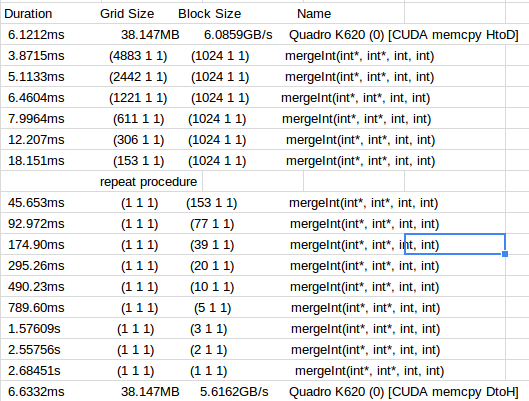
\includegraphics[width=0.8\hsize]{./figures/merge.png}
\end{center}
\caption{{\small {\bf Profiling for parallel merge sort.}  }}
\label{fig-knearest-perf}
\end{figure}
\section*{}
Figure 8 shows the bitonic can exploit as many threads as half of the data size, which make it fast. We think it is the only parallel algorithm
with potential to outperform sequential on our platform. Unfortunately we only make it work up to array with size of 9215. 
\begin{figure}[t]
\begin{center}
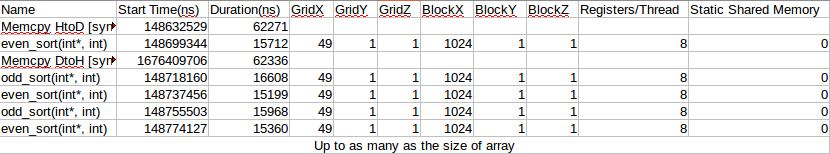
\includegraphics[width=0.8\hsize]{./figures/odd.png}
\end{center}
\caption{{\small {\bf Profiling for parallel even odd sort.}  }}
\label{fig-knearest-perf}
\end{figure}
Profiling shows that all parallel programs written by us all don't take the advantage of shared memory, which is a direction to improve them.
 

\begin{figure}[t]
\begin{center}
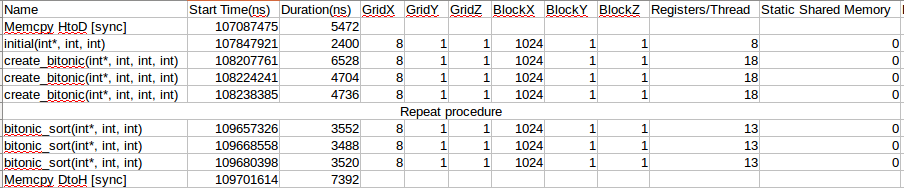
\includegraphics[width=0.8\hsize]{./figures/bitonic.png}
\end{center}
\caption{{\small {\bf Profiling for bitonic sort.}  }}
\label{fig-knearest-perf}
\end{figure}
 




\begin{figure}[t]
\begin{center}
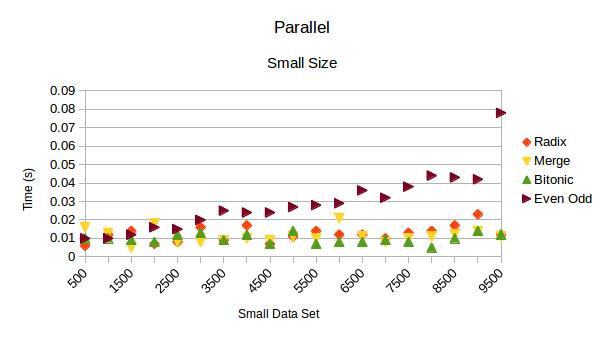
\includegraphics[width=0.8\hsize]{./figures/p_s.jpg}
\end{center}
\caption{{\small {\bf Comparison between different parallel sorting on small size data set.}  }}
\label{fig-knearest-perf}
\end{figure}


\begin{figure}[t]
\begin{center}
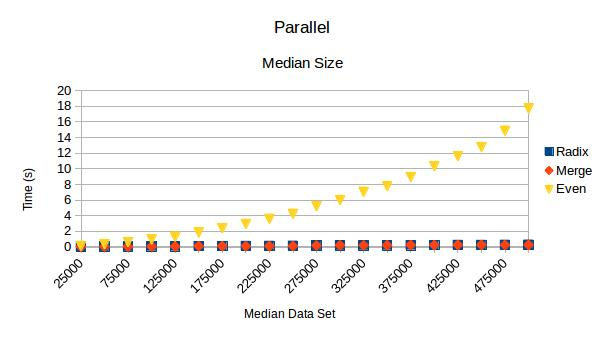
\includegraphics[width=0.8\hsize]{./figures/p_m.jpg}
\end{center}
\caption{{\small {\bf Comparison between different parallel sortings on median size data set.}}}
\label{fig-knearest-perf}
\end{figure}


\begin{figure}[t]
\begin{center}
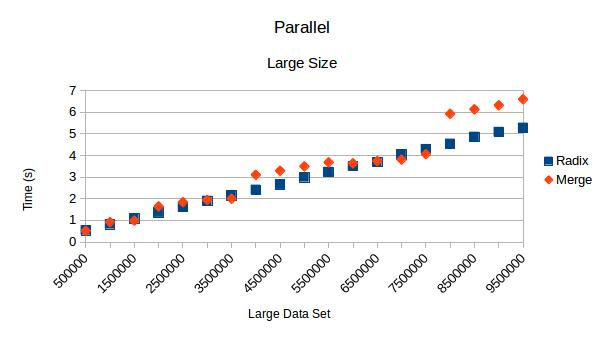
\includegraphics[width=0.8\hsize]{./figures/p_l.jpg}
\end{center}
\caption{{\small {\bf Comparison between different parallel sorting on large size data set.}  }}
\label{fig-knearest-perf}
\end{figure}
\section*{}
Figure 9, 10 and  11 show the Even-Odd sorting algorithm are much still as profiling shows it takes to many rounds to guarantee the data sorted.
Parallel radix is a little better than parallel merge, since on one hand it possesses better characteristics which fit in GPU, on the other hand it
exploit shared memory well.
\section*{}
 
\section{Conclusion}

Although Parallelism is a promising direction to take the advantage of  Moore's law, the programming model is an significant factor affect whether the multiple threads can be used well. In our project most of sorting algorithm don't fit well the GPU programming model. 
 
 \section*{}
 Model ideal for GPU is 
 \begin{itemize}
	\item  Not too small amount of data
	\item Not too big amount of data
	\item Independent data
	\item Intensive calculation with infrequent memory visit
	\item It is best to have  data fit in shared memory 
\end{itemize}
 
 \section*{}
 Parallel radix sort and bitonic sort do possess the characteristics of the ideal model.
 That's why they are relatively faster. 
 \section*{} 
 For radix, there is still a drawback which is it may need dynamically allocate memory. 
\section*{}
 And I think, in our project,  the bitonic is the only one parallel algorithm with potential to outperform sequential algorithms. Unfortunately we only make the bitonic sort work up to
 9215, I need more time to debug. 
 
 


%%%%%%%%%%%%%  THIS IS WHERE THE BIBLIOGRAPHY GOES %%%%%%%%%

% Change the word "template" below to the name of the .bib file you use
 

\end{document}

